\documentclass{eceasst}

\usepackage{minted}
\usepackage{subfig}
\input{frontmatter}

\usepackage{pdfcomment}
\newcommand{\todo}[1]{\pdfcomment[color={0.045 0.278 0.643},icon=Note]{#1}}

\title{Improving reproducibility of scientific software using Nix/NixOS: A case study on the preCICE ecosystem}
\short{preCICE on Nix: A case study}
\author{
Max Hausch\autref{1}\autref{*},
Simon Hauser\autref{1}\autref{*},
Benjamin Uekermann\autref{1}}

\institute{
\autlabel{1} Institute for Parallel and Distributed Systems\\ University of Stuttgart\\ \email{benjamin.uekermann@ipvs.uni-stuttgart.de}\\
%\autlabel{1} \email{st175425@stud.uni-stuttgart.de}\\
%\autlabel{2} \email{st148883@stud.uni-stuttgart.de}\\
\autlabel{*} These authors contributed equally to this work.}

\abstract{
Ensuring reproducibility of scientific software is crucial for the advancement of research and the validation of scientific findings.
However, achieving reproducibility in software-intensive scientific projects is often challenging due to dependencies, system configurations, and software environments.
In this paper, we present a possible solution for these challenges by utilizing Nix and NixOS.
Nix is a package manager and functional language, which guarantees that a package and all its dependencies can be built reproducibly.
NixOS is a purely functional Linux distribution, built on top of Nix, which enables the build of reproducible systems including configuration files, packages, and their dependencies.
We study the potential of Nix and NixOS by a case study on the reproducibility of the preCICE ecosystem.
preCICE is a coupling library for partitioned multiphysics simulations. The ecosystem includes diverse legacy solvers, adapters, and language bindings besides the coupling library itself making it a challenging and representative testcase.
We demonstrate, how to create a reproducible and self-contained environment for this ecosystem and highlight the benefits of using Nix and NixOS.
%In addition, we compare the usability and reproducibility provided by Nix, in the context of preCICE, with two already established high-performance computing (HPC) solutions, Spack and EasyBuild.
%This evaluation enables us to assess the advantages and disadvantages of employing Nix to improve reproducibility in scientific software development within an HPC context.
}

\keywords{Reproducibility, Nix, NixOS, Spack, EasyBuild, preCICE, HPC}

\begin{document}
\maketitle

\section{Introduction}

In scientific research, it is crucial to be able to reproduce and verify results.
Reproducibility ensures that experiments can be repeated and findings can be validated, which is essential for reliable and credible research.
However, achieving reproducibility in scientific software has been a challenge due to complex dependencies, conflicting software environments, and changing software systems~\cite{Dalle_2012}.
Problems arise from dependencies, library versions, and system configurations, leading to inconsistencies across different computing environments.
Traditional approaches to reproducibility, such as manual setup instructions or virtualization techniques, are prone to errors and time-consuming at best.

Many scientists aim to solve this situation using Docker\footnote{\url{https://www.docker.com/}} (e.g.,\cite{koch2023sustainable}),
a software which describes software environments with the help of text files.
Those text files are made up of imperative commands which are run inside of containers, one layer at a time.
The result is several different layers combined into a single output image, which can be instantiated into a running container.
Docker images can be copied to different hosts and should then provide the same environment on different machines.
Those images are usually based on one of the official Docker images\footnote{\url{https://docs.docker.com/trusted-content/official-images/}}, however, which use traditional package managers, such as apt.
When a user then specifies to install the python3 package, for instance, a traditional package manager could yield version 3.8 today, but version 3.9 in a few months.
Full reproducibility can, thus, only be achieved by storing the complete image. Altering a single dependency (e.g., a bugfix) causes a rebuild of the image and, thus, destroys reproducibility.

There are, moreover, commercial, domain specifig solutions to achieve reproducibility, e.g., CodeOcean\footnote{\url{https://codeocean.com/}} mainly for bioinformatics or Weights and Biases\footnote{\url{https://wandb.ai/site}} for machine learning.
With these archiving platforms, experiments can be rerun using technologies such as Docker.
These platforms are closed source, however, such that the source code cannot be reviewed nor adjusted~\cite{koch2023sustainable}.

In past years, the Nix package manager~\cite{Dolstra_2004} and NixOS~\cite{Dolstra_2010}, a Linux distribution built around it, have emerged as promising alternatives~\cite{Devresse_2015}.
Nix allows functional descriptions of dependencies up to fixed versions, thus avoiding the issue described above.
Similar ideas are followed by the popular high performance computing (HPC) package managers EasyBuild~\cite{easybuil6495863} and Spack~\cite{spack7832814}.
All have in common that they rely on scientific software following best practices concerning building and packaging.
Unfortunately, most legacy software projects do not do this.
This is why, for example, the xSDK community~\cite{xSDK2023} tries to set a standard for policies for math software.

In this paper, we analyze how well Nix and NixOS can improve reproducibility of scientific software.
To this end, we study the preCICE ecosystem~\cite{preCICEv2} as an example.
preCICE is a coupling library for partitioned multiphysics simulations.
The ecosystem includes diverse legacy solvers, adapters, and language bindings besides the coupling library itself making it a challenging and representative testcase.
We try to build the complete ecosystem using Nix and verify portability on three different systems.

\section{Background}

In our case study, we use Nix for building and packaging preCICE adapters and their respective solvers.
This chapter gives a short introduction into Nix and preCICE.

\subsection{Nix}\label{sec:nix}

Nix is a purely functional package manager that provides some features to build software derivations reproducibly.
It does so, by recursively calculating a hash over all the inputs of a derivation and its dependencies to ensure the completeness of the whole derivation.
If any of the inputs changes, all dependent derivations will have to be rebuilt.

As Nix is purely functional, it relies on functions that, without side-effects, realize the package derivations.
Inputs to those functions are parameters such as the package version or the location of the source code.
Evaluating and realizing those functions with the same inputs, yields the same outputs.
This is a critical factor where Nix's reproducibility comes from.
Outputs, i.e. the build artifacts, never change after being built once.
Nix builds are sandboxed, meaning that there is no internet access possible during a build.

All contents, including source files and resulting build artifacts, are stored inside the Nix store.
Per default, the Nix store resides in the path \texttt{/nix/store} on the file system.
The naming scheme for the preCICE 2.5.0 package as an example is \path{/nix/store/0a5gw3l\ldots-precice-2.5.0}.
This eases checking the Nix store for integrity and ensures that builds using the same inputs are performed only once.

As each build output references their complete dependency graphs inside the Nix store, they do not interfere with other build outputs, enabling users to have multiple versions of the same software installed at the same time without raising conflicts.
An example of a graphical representation of a dependency graph can be seen in Fig. \ref{fig:nix-graph}.

\begin{figure}
    \centering
    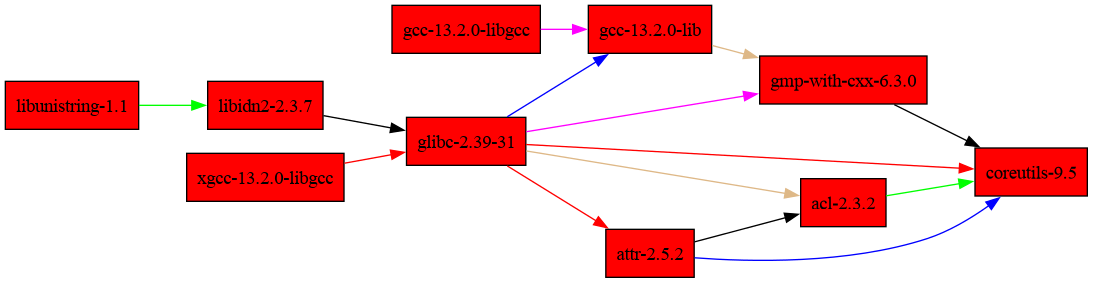
\includegraphics[width=1\textwidth]{figures/coreutils.png}
    \caption{The dependency graph of the coreutils package, generated by \texttt{nix-store --query --graph \$(nix build nixpkgs\#coreutils --print-out-paths) | dot -Tpng -Grankdir=LR -ocoreutils.png}}
    \label{fig:nix-graph}
\end{figure}


Software patches are quite easy to apply in Nix.
One can simply provide a list of \texttt{.patch} files as inputs, Nix will then include the patch files in the build and the calculation of the hash.
Users can override all inputs freely, so every package can be flexibly adjusted to the users needs.


\subsection{preCICE}

preCICE (Precise Code Interaction Coupling Environment) is an open-source software library designed to facilitate the coupling of different computational simulation softwares.
It provides an interface that allows different simulation tools to exchange data and work together in a collaborative manner, enabling multi-physics as well as multi-scale simulations.

Many scientific simulations require complex combinations of multiple solvers, each specialized in a particular aspect of the problem.
For example, in fluid-structure interaction problems, where fluid flow interacts with deformable structures, separate solvers can be used to model the fluid dynamics and structural mechanics.
preCICE acts as a bridge between all solvers participating in the simulation, allowing them to exchange data and synchronize their computations.

preCICE offers a flexible and generic framework for coupling simulations.
It supports a wide range of solvers, including finite element, finite volume, and particle-based methods.
The library provides methods for interpolating data between meshes, managing communication between solvers, and handling time stepping and convergence.
It can handle different types of coupling scenarios, such as one-way or bidirectional couplings, loose or tight couplings, and static or dynamic meshes.
The core principle of preCICE's functionality is shown visually in Fig. \ref{fig:precice}.

\begin{figure}
    \centering
    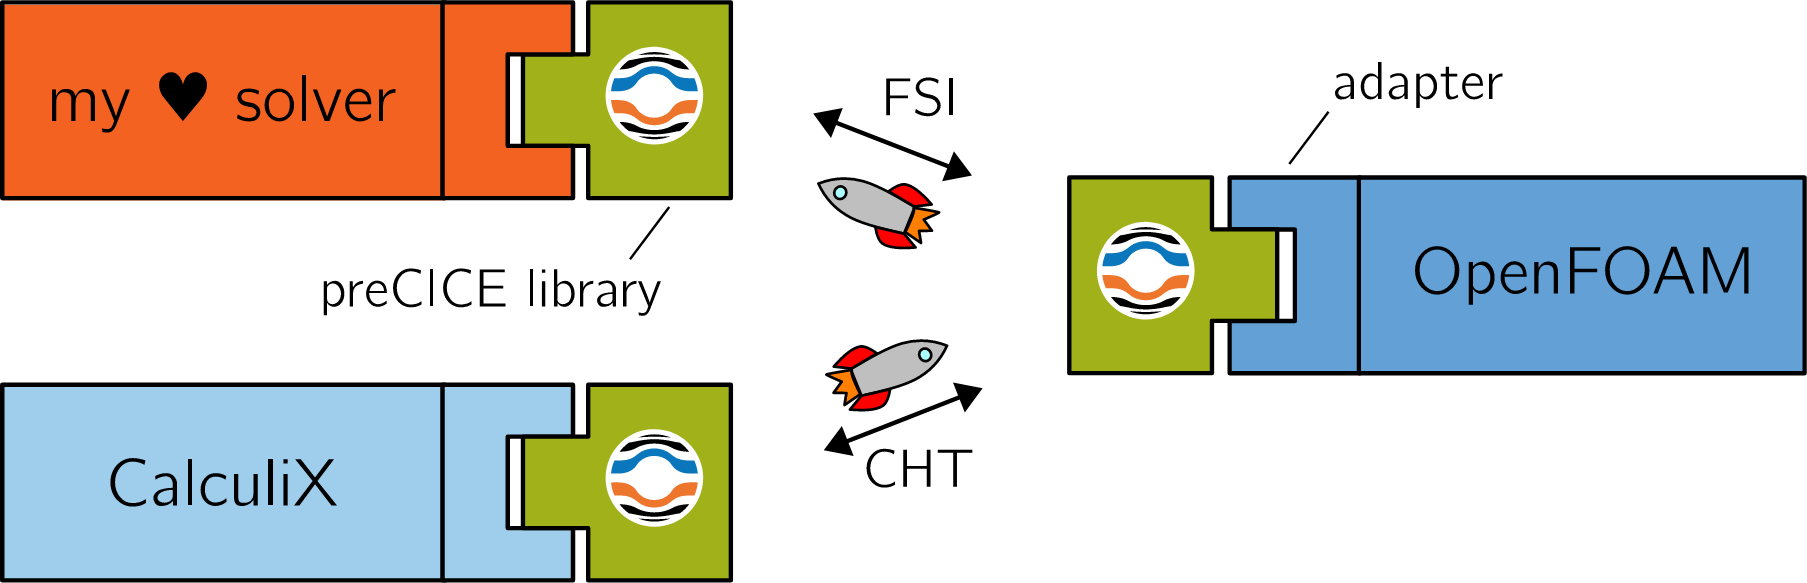
\includegraphics[width=0.5\textwidth]{figures/precice.png}
    \caption{A visual representation on how preCICE works in principle, see: \url{https://precice.org}}
    \label{fig:precice}
\end{figure}

One main idea behind preCICE is to enable the combination of existing simulation tools without requiring significant modifications to their original source code.
Instead, preCICE provides an abstraction layer that sits between the individual solvers, allowing them to communicate and exchange data efficiently.
This approach promotes code reusability and reduces the effort required for coupling simulations.

preCICE is an open-source project, that means its source code is freely available and can be modified and distributed by the community.
This fosters collaboration and encourages the development of new features and improvements by researchers and engineers worldwide.

Overall, preCICE simplifies the process of coupling different simulation programs, enabling the simulation of complex multi-physics problems.
It promotes interoperability, code reusability, and collaboration, making it a valuable tool in various engineering and scientific domains.

\section{Results}

To see how well Nix can be used to build and package scientific software reliably and reproducibly, we conduct a case study in the context of the latest preCICE distribution~\cite{preciceDistribution}, currently preCICE \texttt{v2211.0}.
The preCICE distribution consists out of the preCICE core library, as well as some tools, bindings, adapters, tutorials, the website and documentation, and the preCICE VM\footnote{\url{https://precice.org/installation-distribution.html}}.
Table \ref{table:label-distribution} shows an overview over all packages provided by the preCICE distribution and their respected versions.

\begin{figure*}[!t]
  \normalsize
  \caption{Overview of preCICE distribution}
  \label{table:label-distribution}
  \centering
  \begin{tabular}{|c|c|c|c|}
    \hline
    \bfseries Package & \bfseries Type & \bfseries Build System & \bfseries Version \\ \hline
    precice & library & cmake & 2.5.0 \\ \hline
    fortran-module & bindings & make & 9e3f405 \\ \hline
    julia & bindings & julia & v2.5.0 \\ \hline
    matlab & bindings & matlab build script & v2.5.0.0 \\ \hline
    pyprecice & bindings & setup.py & 2.5.0.1 \\ \hline
    config-visualizer & tooling & setup.py & 60f2165 \\ \hline
    precice-aste & adapter & cmake & 3.0.0 \\ \hline
    dealii & solver & cmake & 9.4.1 \\ \hline
    precice-dealii-adapter & adapter & cmake & dbb25bea \\ \hline
    precice-calculix-adapter & adapter & makefile & 2.20 \\ \hline
    fenics & solver & cmake + setup.py & 2019.1.0 \\ \hline
    precice-fenics-adapter & adapter & setup.py & 1.4.0 \\ \hline
    precice-dune & adapter & scripts + cmake & 2.8.0 \\ \hline
    Dune-fem & library & setup.py & 2.8.0.0 \\ \hline
    code-aster & solver & custom build system in python & 14.6.0 \\ \hline
    openfoam & solver & wmake/Allwmake & 2206 \\ \hline
    openfoam-adapter & adapter & wmake/Allwmake & 1.2.1 \\ \hline
    Precice-su2 & solver + adapter & patch script + autoconf & 6.0.0 \\ \hline
    Nutils & library & setup.py & 7.0.0 \\ \hline
  \end{tabular}
\end{figure*}


We are mainly interested in the tools, adapters including their solvers and the preCICE VM.
For each of these entities, we present possible challenges, how to circumvent those and also comment on how software can be designed to make it as easy as possible for other users to build and package the software in question.

\subsection{preCICE}

The preCICE library itself is already available in the nixpkgs repository, so we do not have to package the software.
Looking at the package definition and the preCICE source code, the library is quite easy to build and package as it uses CMake as a build system.

\subsection{Tools}

The preCICE distribution comes with a few tools that ease working with preCICE.
They are mainly meant for debugging and visualizing several aspects of preCICE and preCICE configuration files.

\subsubsection{ASTE}

This package is a collection of tools that help in development of new adapters.
It stands for Artificial Solver Testing Environment, so it allows for debugging adapter mapping setups and other similar tasks.

ASTE\footnote{\url{https://github.com/precice/aste}} needs VTK9\footnote{\url{https://vtk.org/}}, a visualization toolkit, that is built without python support in the nixpkgs repository to reduce compilation time.
However, this feature is needed for ASTE.
As already mentioned, Nix allows easy overriding of inputs, so in this case, we can look at the package definition of VTK.
The parameter \texttt{enablePython} can simply be set to \texttt{true}, then we also need to supply the version of python we want to compile against, so in our case \texttt{python = python3;}.

After enabling python support in VTK, the package can be built without further modifications.

Only for testing, we additionally need to replace the absolute paths to \texttt{/bin/bash} and \texttt{/usr/bin/time}, then all tests succeed without any problems.

\subsubsection{config-visualizer}

The precice-config-visualizer\footnote{\url{https://github.com/precice/config-visualizer}} package can be used to generate images that represent a specified preCICE config file to check graphically what is configured in the file.

This tool is already packaged upstream, so we can just use it.
As it is a python package, it is quite easy to build with Nix, so the package definition is straight forward.

\subsection{Bindings}

Bindings are used to offer interfaces to other programming languages.

\subsubsection{python-bindings}

The \texttt{pyprecice} package is already available upstream, however it is broken and does not compile as it is not able to find the python module \texttt{pkgconfig}.
After adding this single dependency as an input to the package definition, the python package builds and can be used as expected.

\subsubsection{Julia-bindings}

Julia~\cite{bezanson2017julia} support in NixOS is currently still in its early stages and cannot be declaratively be defined by Nix\footnote{\url{https://github.com/NixOS/nixpkgs/issues/20649}}.

\subsection{Adapters}

A preCICE distribution comes bundled with several adapters, that are currently not in the upstream nixpkgs repository.
Many of the adapters use solvers that are not packaged in the upstream repo as well, so in order to get the adapters to work, these also have to be packaged and sometimes patched.

\subsubsection{CalculiX}

The preCICE adapter for CSM code CalculiX~\cite{Uekermann2017_Adapters}, requires the original CalculiX source code and provides a new Makefile in the adapter repository.
By default, this Makefile expects the source code to reside in \texttt{\$HOME}, but it is possible to override this location with a make variable.
It then builds the original code and the adapter code together, resulting in a combined binary.

The Makefile also has hard-coded dependency location for \texttt{SPOOLES}, \texttt{ARPACK} and \texttt{YAML} so these need to be replaced with the equivalent \texttt{pkg-config} calls, because Nix does not have these dependencies at the hard-coded locations, and generally only finds dependencies with \texttt{pkg-config}.
Additionally, there is no \texttt{install} target provided by the Makefile so the resulting binary needs to be installed manually by copying it to \texttt{\$out}.\\

\subsubsection{code\_aster}

The code\_aster preCICE adapter~\cite{Uekermann2017_Adapters} is a python file that needs to be placed in the code-aster lib directory.
For this, the code\_aster solver needs to be packaged at the latest stable version 14.6.
It uses a custom build system based on a \texttt{setup.py} file, that invokes build and install phases for dependencies and in the end for the solver itself.

The stable package also distributes the dependencies as pinned tarballs.
On Nix almost none of these dependencies, complete the build stage with the \texttt{setup.py}, so we need to pull them out, package them separately as Nix packages and configured the build system with a \texttt{setup.cfg}.
In this file, we are able to disable the installation of the pinned dependencies and provide paths to the dependencies instead.

With this approach, we disable HDF5, as it is already packaged in the upstream nixpkgs repository, even at the required version 5.1.10.
HDF5 is packaged with multiple outputs.
One package, \texttt{out}, contains the libraries and binaries and another, \texttt{dev} contains the header files, this is, because most of the time, users installing HDF5 only need the libraries and binaries, and it helps to reduce installation size of this rather large package.
Additionally, code\_aster requires medfile and scotch, that are both available upstream and can be used as a dependency.

Another dependency, that is also provided by code\_aster is metis, that partially builds, so we do not replace this dependency, but we need to fix the second part of the build, including the metis programs such as gpmetis, ndmetis, mpmetis and more.
The issue is that in the \texttt{CMakeLists.txt} for the metis programs \texttt{link\_directories} is hard-coded to \path{/home/karypis/local/lib}.
After removing this line, it also installs, so to resolve this issue in the buildPhase, we unpack the metis tarball, remove this line with \texttt{sed} and then repack the directory.

The last 2 dependencies, are not available and need to be packaged, this includes mumps and tfel, also known as mfront.

Mumps builds using a Makefile and can be configured using Makefile.inc, by default it provides a couple of these configurations for systems such as Ubuntu, so we use one of these provided configuration files to write our own custom config file.
It defines the location for dependencies such as scotch, metis, parmetis, liblapack, blas, scalapack and blacs.
Almost all the dependencies, are available upstream, but we need to recompile scotch with additional build flags, \texttt{scotch ptscotch esmumps ptesmumps} using Nix overrideAttrs feature.
For packaging blacs, that also uses a Makefile, we configure the build using a custom \texttt{Bmake.inc} file, that is used to set compiler flags, the path to the mpi and bash installation.

The last missing dependency for code\_aster, tfel, uses CMake as a build system making it trivial to package it with Nix and we only have to set a couple of CMake flags.

After successfully packaging all dependencies, the build phase of code\_aster completes, but the installation part has another issue, that also affects new versions of Ubuntu and other distributions that use a python version greater than 3.9.
There is a forum post without any resolution from the developers or the community, so we need to manually patch the bug.

The issue is that the custom build system does not correctly calculate the python site-packages directory because it unconditionally slices the first 3 chars from \texttt{sys.version}, that works if your version is 3.9.x but not with 3.10.x because then the code calculates \path{lib64/python3.1/site-packages} rather than the expected \path{lib64/python3.10/site-packages}.

After patching this bug code\_aster successfully installed into \texttt{\$out/14.6/}, so we move around some files until we have a valid directory structure with \texttt{\$out/bin}, \texttt{\$out/lib} and we provide symlinks for \texttt{\$out/14.6/} and \texttt{\$out/stable/} as code\_aster expects configuration files in these directories.

Last but not least, we can copy the code\_aster adapter at the required location.\\

\subsubsection{deal.II}

In order to package this adapter, we first need to package deal.II~\cite{dealII95}, that uses CMake as build system and works without any adjustments.
The same applies for the adapter, that also uses CMake and needs preCICE as a dependency.
When supplied with the inputs, the adapter builds without any problems.
As an example for the Nix language, you can see the abbreviated Nix code for the dealii.II adapter in Fig. \ref{lst:dealii-adapter-nix}.\\

\begin{figure*}
    \normalsize
    \begin{minted}{nix}
{ lib, stdenv, fetchFromGitHub, cmake,
  precice, dealii, enable3d ? false }:

stdenv.mkDerivation rec {
  pname = "precice-dealii-adapter";
  version = "unstable-2022-09-23";

  src = fetchFromGitHub {
    owner = "precice";
    repo = "dealii-adapter";
    rev = "dbb25...8367c";
    sha256 = "sha256-pPQ2...2jlflgUE=";
  };

  nativeBuildInputs = [ cmake ];
  buildInputs = [ precice dealii ];

  cmakeFlags = lib.optionals enable3d [
    "-DDIM=3"
  ];

  installPhase = ''
    mkdir -p $out/bin
    cp elasticity $out/bin/elasticity
  '';
}
    \end{minted}
    \caption{A sample of Nix code used to package the dealii-adapter, see: \url{https://github.com/precice/dealii-adapter/}}
    \label{lst:dealii-adapter-nix}
    \hrulefill
    \vspace*{4pt}
\end{figure*}

\subsubsection{DUNE}

The DUNE~\cite{bastian2020dune} package uses a combination of CMake files and custom build scripts making the build process quite tedious.
This might be an issue because of the ongoing migration to CMake from autotools and might be resolved in the future.

It is also a minor issue that the dune-project is a collection of repositories rather than a monorepository, because users have to correctly clone all repositories so the build system finds all relevant information.
We clone all of the required dune repos into a directory and additionally clone the adapter into the same directory.

For the build and install, process we need to manually set \texttt{\$DUNE\_CONTROL\_PATH} and \texttt{\$DUNE\_PY\_DIR} environment variables, both variables also need to be set at runtime.
Additionally, we need to patch the python install process because the current CMake file that handles this install tries to access the internet with \texttt{pip install}.
This is not allowed in Nix' sandboxed builds.
Therefore, we need to patch the \texttt{pip} command with the options \texttt{--no-cache-dir --no-index --no-deps --no-build-isolation} and remove the \texttt{--upgrade} option.\\

\subsubsection{FEniCS}

We are explicitly referring to the legacy version of FEniCS~\cite{fenics} here, not the newer and still experimental FEniCSx.
This adapter~\cite{Rodenberg2021} uses the open source computing platform FEniCS, that is already packaged within nixpkgs, to provide preCICE support.

Although it is available, not all features the adapter needs are enabled, including PETSc support.
To fix this, we need to package PETSc4py, that provides python bindings for PETSc and is not present in the upstream nixpkgs repository.
The build process is possible without any issues, because it uses the internal \texttt{buildPythonApplication} build tool, but we need to add the additional build optional \texttt{build\_src --force} because the cython code needs to be rebuilt.
We also are not able to enable tests for this package because tests depend on OpenMPI and the network, that is not available within the Nix build sandbox.

After this, we can specify PETSc4py as dependency for FEniCS and can enable support for this feature.

Building the adapter with Nix is now possible with \texttt{buildPythonPackage} and does not require any special workarounds.
A majority of the \texttt{pytest} ran successfully, but two tests failed inside the Nix sandbox, that means all tests needed to be disabled.\\

\subsubsection{OpenFOAM}

There are two flavors of OpenFOAM, we are referring to the OpenFOAM fork of OpenCFD Ltd\footnote{\url{https://www.openfoam.com/}}.

OpenFOAM uses its own custom build system called \texttt{wmake} that is sometimes called with a wrapper script called \texttt{Allwmake}.
The build system sets 36 environment variables that are set by wmake, one step at a time by checking several parameters, e.g. the cpu architecture or the location of the source code, and concatenating some other environment variables together.

Allwmake and wmake rely on these environment variables to be set, as otherwise the tools will exit with a warning.
During runtime, before running any OpenFOAM commands, a small wrapper script has to be started that sets all relevant environment variables, or a user has to manually source a file inside the installation directory of OpenFOAM.
OpenFOAM uses modules for extensibility and flexibility that need the source code of OpenFOAM and also require wmake as a build tool.

For Nix, these properties are rather unfortunate.
To compile OpenFOAM with Nix, we first need to patch the shebangs\footnote{\url{https://foldoc.org/shebang}} of wmake to make it run during the build.
Secondly, we render a shell script we call \texttt{set-openfoam-vars} that exports all necessary environment variables to the current shell session.
At the time of writing, all parameters such as the processor architecture are hard-coded for simplicity reasons but could be parametrized based on the Nix inputs to allow for optimized builds.
During the buildPhase, the rendered script will be sourced to set all variables, e.g. so the \texttt{OPENFOAM\_SRC\_PATH} points to \texttt{/build/openfoam} being the default location for Nix builds inside the sandbox.
After sourcing the script, the single command \texttt{./Allwmake -j -q} is sufficient to start the build.

The installPhase then simply copies the necessary files and directories to \texttt{\$out}, replaces the mock \texttt{OPENFOAM\_SRC\_PATH} by the value of \texttt{\$out} and creates a wrapper for the \texttt{openfoam} shell script.

As the preCICE OpenFOAM-adapter~\cite{OpenFOAMpreCICE} is an OpenFOAM module, the derivation of the adapter needs OpenFOAM and wmake as build inputs.
The correct environment variables have to be set again, but this is rather easy now, as we have the \texttt{set-openfoam-vars} script that we can simply source during the buildPhase.
The last thing we need to change before launching the build with Allwmake is to set the target directory for the adapter.
A single shared library that can be copied to \texttt{\$out/lib/} is the only output for this build.

Debug and timing modes for the adapter can simply be enabled by setting the \texttt{debugMode} and \texttt{enableTimings} inputs to the derivation to true.

OpenFOAM is available on Spack and EasyBuild that both patch the OpenFOAM source files as those tools also have to set environment variables to make a build compatible with wmake.\\

\subsubsection{su2-adapter}

This package is a preCICE adapter~\cite{Uekermann2017_Adapters} for the CFD code SU2 and extends the original SU2 source code by patching the files.
For this, the adapter provides a custom script that needs to be executed before the build phase.
Nix offers the patchPhase that allows us to run the script in this phase and patch the original source, after that the \texttt{stdenv} automatically recognizes that the repository uses autotools for building the software and runs the configurePhase.

We additionally needed to add the two configureFlags \texttt{--with-include} and \texttt{--with-lib} to the preCICE install directory because otherwise autoconf does not find the preCICE installation directory.

\subsection{preCICE VM}

The current preCICE VM is built on top of Vagrant\footnote{\url{https://www.vagrantup.com/}} using Ubuntu as a base image.
When it is run for the first time, it further installs software, compiles programs and the preCICE tutorials\footnote{\url{https://github.com/precice/tutorials/}}.
This inherently breaks reproducibility as the VM fetches files from the internet that are at this very point in time the ``latest'' version, e.g. the \texttt{main} branch of the preCICE repository.

Nix comes with the built-in functionality of producing qemu\footnote{\url{https://www.qemu.org/}} VM images.
We used Nix to define a VM image with NixOS as a base, that can be built reproducibly.
The image contains all the adapters and solvers from the case study and some additional custom tools that can only be seen in the official VM, such as the \texttt{preciceToPNG} command.
Also, we generate an iso and a Vagrant VirtualBox file of the VM as additional outputs.

\begin{sloppypar}
Most of the functionality that can be found in the official VM is also available in our NixOS VM and all preCICE tutorials could be run successfully, except \texttt{turek-hron-fsi2} as the tutorial needs \texttt{swak4foam}, an add-on to OpenFOAM, we were not able to package, \texttt{flow-over-heated-plate-steady-state} as the manual steps involved were unclear, \texttt{partitioned-heat-conduction-complex} and \texttt{partitioned-heat-conduction-direct} as the \texttt{mshr} python dependency was missing.
\end{sloppypar}

\section{Discussion}

After detailing the challenges of building and packaging each solver and their respective adapter, we want to discuss some common points between these scientific software packages.
preCICE, as a multi-component research software, covers many different simulation codes and therefore provides a good overview over different kinds of packages, making this case study representative for multi-component research software.\\

Generally speaking, there are major gaps regarding the ability to successfully package the software between each different software solution that can be traced back to the build system.
Custom build systems require an disproportional amount of additional work to make them runnable on any system.
OpenFOAM and Allwmake are prime examples of these issues because now package managers have to understand a whole new build system for exactly one package in order to successfully package it and make it easily available to users.
It is also worth mentioning that writing your own custom build system, requires additional time to maintain this build system, that could have been spent working on the software itself.
Packages that use common, industry proven package managers, such as CMake and autotools make it easier for developers of the software to build their software as well as package managers to package it.
These build tools, generally also provide interfaces for dependency management that can be used to tell users and package maintainers what dependencies are needed, and it is usually better than only documenting required dependencies, because documentation needs to be kept in sync with the underlying code.
They also generally already provide proven interfaces for configuring packages with additional features, and these also might be self documenting.

The authors of the xSDK\footnote{\url{https://xsdk.info/}} came to a very similar conclusion.
Their goal is to ``identify, adapt, and adopt best practices in software engineering'' and ``to provide the foundation of this extensible scientific software ecosystem''~\footnote{\url{https://xsdk.info/}}.
To achieve this they provide a list of package policies~\cite{xSDK2023}, that for example specifies as mandatory policy that packages ``must support portable installation through Spack''~\cite{xSDK2023} and that all packages ``should have a build system that is appropriate for the language''~\cite{xSDK2023}, that includes CMake and autoconf as examples.
If a package supports all these policies, they can be added to the growing list of packages in the xSDK, that currently among other things include PETSc, deal.ii and preCICE.
These packages are already part of nixpkgs, or it is easy to provide a package for them because they support portable installation, meaning installation into custom prefixes such as nix store paths, and common build systems such as CMake and autoconf.

Another finding is, that is also addressed in xSDK through portable installations, is the requirement to install software to be installed into \texttt{\$HOME} or requires files to be located at a specific location on your file system.
Most of the time, it is possible to work around this, but there are already available solutions for dependency management.
Both, the CalculiX-adapter and SU2-adapter do require the original source code to be present as they add new features on top or patch the source code.
The current solution of the user cloning the code at the specific location works, but it might be better to look into submodules because that also allows the developers to pin the version more easily rather than documenting it, as that could more easily lead to user error, when they try to package and install the adapters.

Additionally, hard-coding libraries to \texttt{/usr/lib} and \texttt{/usr/include} might work on one distribution, but might make it hard or even impossible to install a package on a different distribution or even a later version of the same distribution.
Solutions such as \texttt{pkg-config} that can be configured, so it finds libraries outside the common paths, should always be preferred and work out of the box with the common paths such as \texttt{/usr/lib}.

With Nix' dependency management, we can easily copy the package definitions we just wrote onto different systems, e.g., entirely different Linux distributions, and execute the build of the closures there.
Building the same closures yields the same outputs, as already described in section \ref{sec:nix}.

\section{Conclusion and Outlook}

In conclusion, the case study was a success, as it has shown that packaging of scientific software with Nix is possible, but it is not as trivial as expected.
Once the software is packaged, it is quite easy to be used and combined in environments with other packaged softwares without conflicts.
The packaged adapters and solvers work well together with the preCICE library and simulations can be run successfully, so this specific case study has shown the potential of Nix in the domain of scientific software.
More research has to be done on the topic, yet we are positive about possible future results in Nix abilities and its flexibility in similar domains.

The majority of the packages required some solution for a fundamental issue within the scientific software or its build system that is not solvable for none experienced Nix users, making it hard for people to use it even for their own software.
Nix itself also is partly at fault, because of its unique nature, that every piece of software lies within \texttt{/nix/store} and that each store path is its own-isolated tree based on the Filesystem Hierarchy Standard (FHS).
But it is worth mentioning that not only Nix would benefit from more streamlined build systems and packaging, because both Spack and EasyBuild do something similar for their packages, where each package also lies in its own FHS.
The work of the xSDK people and their policy might be a step in the right direction but looking at the current list of software that is available within the latest xSDK release, 26 libraries, indicates that it is an uphill battle that might take several more years, especially if we consider that the first release happened in 2016.

The Nix code for the packages for the case study on the preCICE adapters, solvers and the preCICE VM is available online in a git repository at \url{https://github.com/precice/nix-packages/} with a more in-detail report that also includes a comparison between Nix, Spack and EasyBuild and a evaluation of Nix on HPC~\footnote{\url{https://github.com/precice/nix-packages/releases/tag/initial-paper-release}}.

While this case study and this comparison has provided valuable insights into the topic of reproducible software, there are still numerous unanswered questions that merit further investigation.
This includes a full evaluation if there are performance improvements using a full impure system rebuild, with \texttt{-march=native} compared to only rebuilding the package at hand.
It would also be interesting to look at trying to reproduce a nixpkgs commit from 10 years ago, and if there might be issues and incompatibilities with newer Nix versions, that currently get released in a 6 weeks time windows.

Last but not least, it would be interesting to investigate Nix and NixOS on HPC even more.
It would be interesting to see how an HPC cluster completely build on NixOS could improve maintaining the HPC cluster, with slurm already being available as a nixpkgs package and module providing a systemd service.

Finally, it would be interesting to investigate a nix store that is shared between users and how it might optimize the amount of storage needed for a cluster as each user is not required to rebuild the same package in their respective home directories.

This summary shows, how diverse and complex Nix is, and how much more opportunities there are to be researched in the future.

\nocite{*}
\bibliographystyle{eceasst}
\bibliography{paper}

\end{document}
